\section{DBpedia}

\begin{frame}
\frametitle{DBpedia}


\begin{minipage}{0.7\textwidth}
\begin{itemize}
  \item DBpedia gathers structured information from Wikipedia
	\begin{itemize}
	  \item infoboxes
	  \item tables, lists
	  \item images
	  \item categories
	  \item links
	  \item geocoordinates
	\end{itemize}
	\item[]
  \item english version currently describes 4 million things
  \begin{itemize}
    \item 832.000 persons, 639.000 places,
    372.000 creative works, 209.000 organizations, 226.000 species, 5.600
    diseases
    \end{itemize}
\end{itemize}
\end{minipage}
\hfill %wichtig, hier keine leerzeile im code
\begin{minipage}{0.25\textwidth}
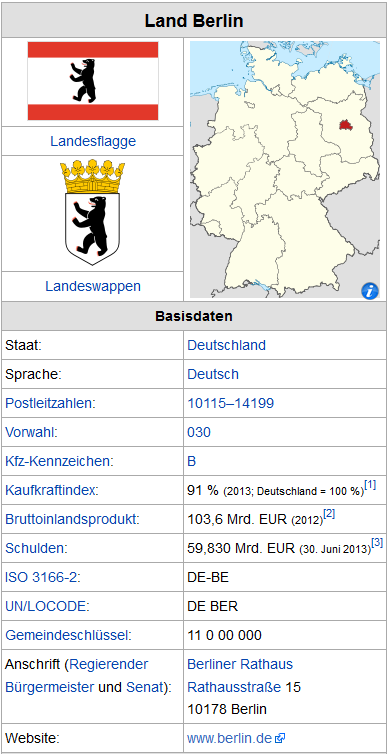
\includegraphics[scale=0.25]{img/berlin_infobox.png}
\end{minipage}
\end{frame}

\begin{frame}
\frametitle{Size}
\begin{itemize}
  \item 119 localized versions, in total:
  \begin{itemize}
    \item  12.6 million unique things
    \item 24.6 million links to images
    \item 27.6 million links to external web
    pages
    \item 45.0 million external links into other RDF datasets
    \item 67.0 million links to Wikipedia categories
    \item 41.2 million YAGO categories
  \end{itemize}
  \item[]
  \item Linked Data!
\end{itemize}
\end{frame}

\begin{frame}
\frametitle{Linked Open Data Cloud}
\centering
\begin{figure}
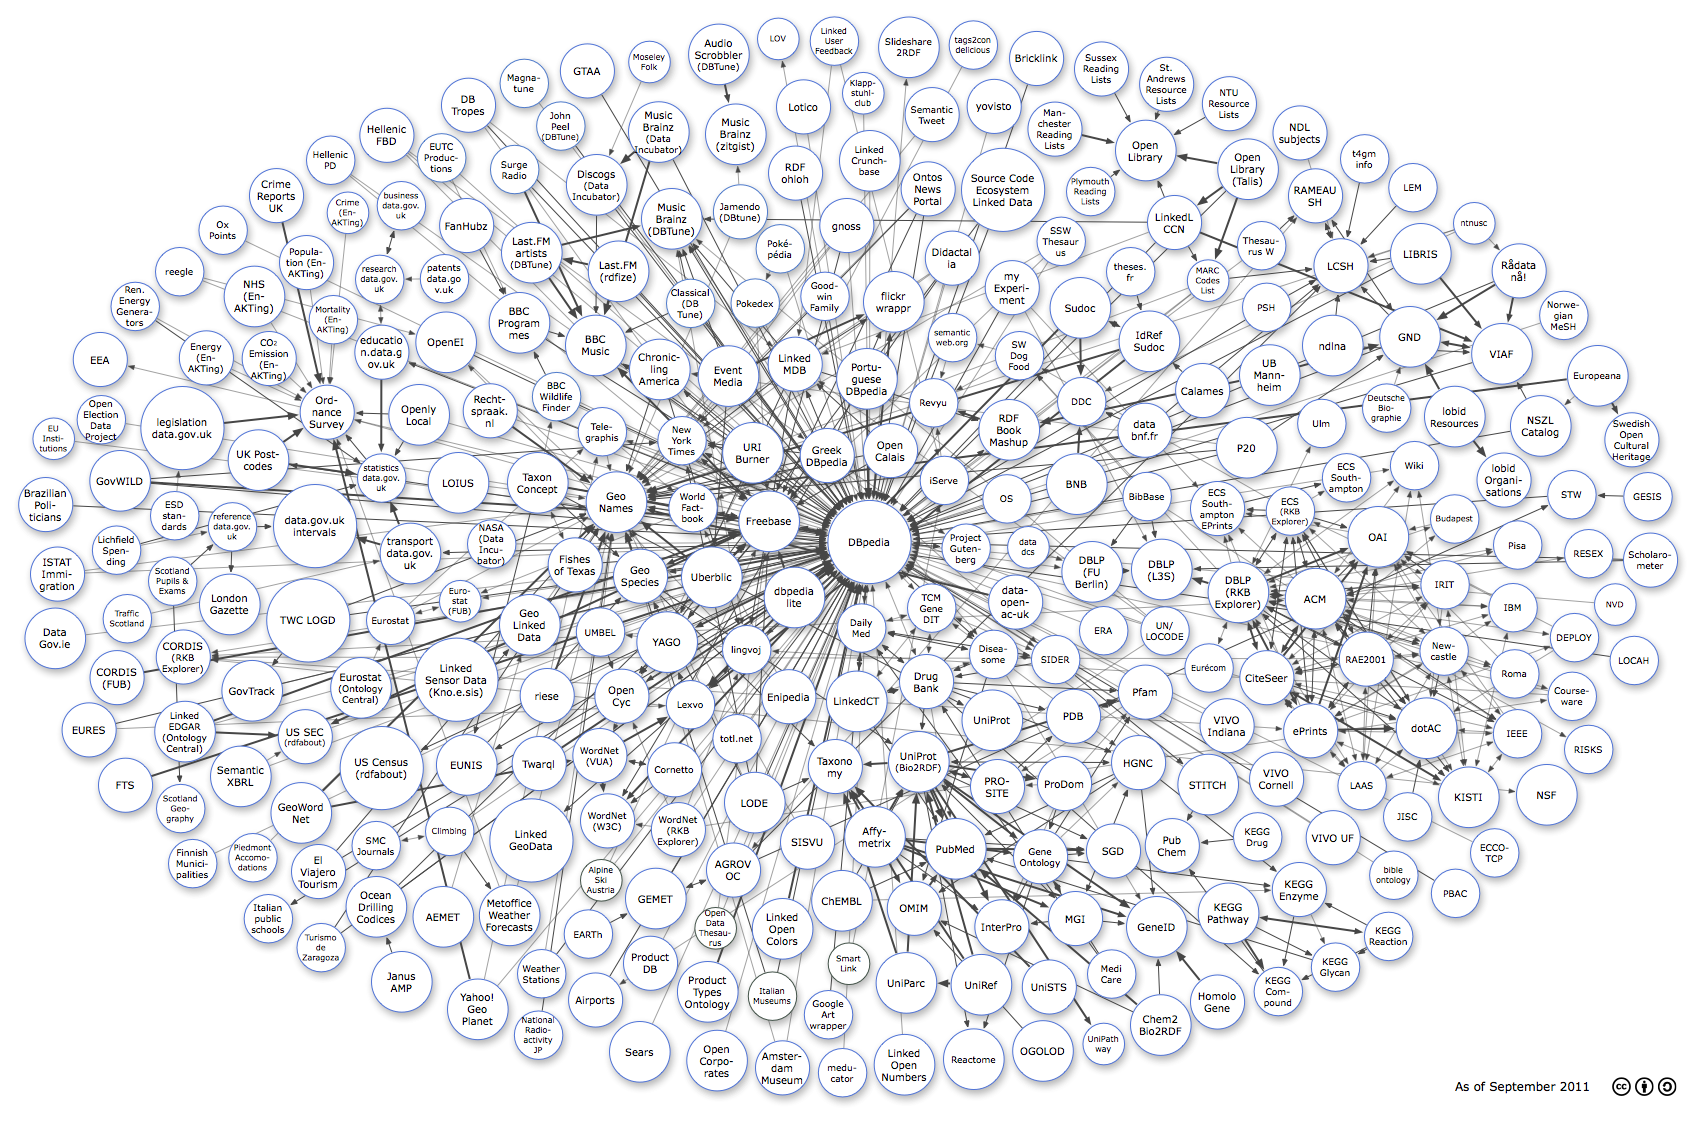
\includegraphics[scale=0.17]{img/lod-cloud.png}
\end{figure}
\small Linking Open Data cloud diagram, by Richard Cyganiak and Anja Jentzsch.
\url{http://lod-cloud.net/} (9/2011)
\end{frame}


\begin{frame}
\frametitle{Usage}
\begin{itemize}
  \item Use cases

	\begin{itemize}
	  \item sophisticated queries against Wikipedia
	  \item use data for web pages
	  \item ``geographic applications'' (connected to other geographic services
	  like Geonames, CIA World Factbook, \ldots)
	  \item annotate web content (multi-domain ontology)
	  \item many links to other datasets and vice versa
	\end{itemize}
	\item[]
	\item Already used at
	\begin{itemize}
	  \item BBC
	  \item Amazon Datasets
	 \end{itemize}
\end{itemize}
\end{frame}


% technology
\begin{frame}
\frametitle{Access and Representation}
\begin{itemize}
  \item De-referencable URIs in the form of
  \url{http://dbpedia.org/resource/[Name]}
  \item Information is represented in RDF format (or CSV)
  \item Provides a SPARQL endpoint
  \item Classifications:
  \begin{itemize}
    \item Wikipedia Categorization
    \item YAGO Classification
    \item WordNet Synset Links
  \end{itemize}
  \item Links to official homepages
  \item Owl:sameAs links (to DBpedia and external documents)
  \item Properties (rdfs, owl, foaf, dc, \ldots)
  
\end{itemize}
\end{frame}

\begin{frame}
\frametitle{Application - SNORQL}
\begin{itemize}
  \item Online SPARQL Explorer for DBpedia
  \item \url{http://dbpedia.org/snorql/}
  \item Example \ldots
\end{itemize}
\end{frame}


\begin{frame}
\frametitle{Application - DBpedia Spotlight}
\begin{itemize}
  \item Transforms any text into DBpedia-annotated text
  \item Web Application \url{http://dbpedia-spotlight.github.io/demo/}
  \item RESTful Web Service \url{http://spotlight.dbpedia.org/rest/spot}
  \item Result can be returned in XML, JSON, HTML, RDFa or NIF 
  \item Example \ldots
\end{itemize}
\end{frame}
